
%(BEGIN_QUESTION)
% Copyright 2015, Tony R. Kuphaldt, released under the Creative Commons Attribution License (v 1.0)
% This means you may do almost anything with this work of mine, so long as you give me proper credit

Dette wattmeteret måler effekt i én fase av et trefasesystem ved å måle både linjespenning og linjestrøm via instrumenttransformatorer. Nominell linjespenning i dette anlegget er 4160 V AC, og strømmen kan komme opp mot 180 A AC ved full last:

$$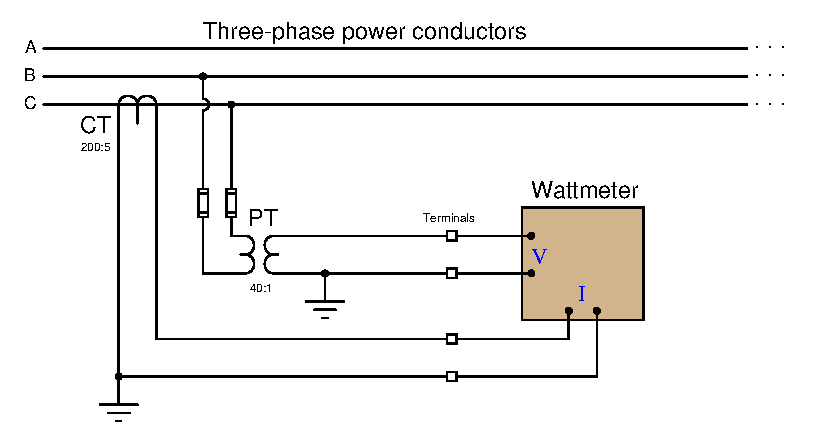
\includegraphics[width=15.5cm]{i01212x01.eps}$$

Hva må du gjøre for å kontrollere kalibreringen av dette wattmeteret? Lag en trinnvis prosedyre du kan gi til en annen tekniker for å simulere presise elektriske effektverdier inn på wattmeteret, med sikkerhet som høyeste prioritet. Merk: Du har ikke lov til å koble ut effekt i trefasesystemet under testen; den må utføres ``live''.

\vskip 10pt

Effekten i et balansert trefasesystem er gitt av følgende formel:

$$P = \sqrt{3} V_{linje} I_{linje}$$

\vskip 20pt \vbox{\hrule \hbox{\strut \vrule{} {\bf Forslag til sokratisk diskusjon} \vrule} \hrule}

\begin{itemize}
\item{} En viktig sikkerhetsregel ved arbeid i spenningssatt krets er ``one-hand rule''. Forklar hva regelen innebærer, og hvordan den brukes i en situasjon som denne.
\item{} Når du løsner skruene på en terminalblokk for å koble fra PT-signalet, bør du ta av lederne på venstre side av terminalene (som vist i diagrammet) eller høyre side, eller spiller det ingen rolle?
\item{} Å koble fra et wattmeter fra spenningssatte instrumenttransformatorer innebærer betydelig risiko. Foreslå hvordan denne prosedyren kan gjøres sikrere med egne ``test switches'' på signalledningene, slik at teknikeren kan isolere wattmeteret uten å bruke skrutrekker på spenningssatte terminaler.
\item{} Anta at PT-utgangen er 113.6 V RMS og CT-utgangen er 2.9 A RMS. Hvor mye effekt tilsvarer dette i trefasesystemet?
\item{} Hvorfor er sekundærkretsene til begge instrumenttransformatorene jordet?
\item{} Anta at potensialtransformatoren har pålitelighet 0.9995 og strømtransformatoren 0.9998. Beregn sannsynligheten for at wattmeteret mottar korrekte data fra begge for effektberegning.
\end{itemize}

\underbar{file i01212}
%(END_QUESTION)





%(BEGIN_ANSWER)

PT-utgangen er vanligvis på eller under 120 V AC. CT-utgangen er vanligvis på eller under 5 A AC. En sentral del av prosedyren er derfor hvordan disse spenning- og strømnivåene kan simuleres nøyaktig inn på wattmeteret.

\vskip 10pt

Ved linjespenning 4160 V skal en PT med forhold 40:1 gi $1 \over 40$ av dette (104 V AC) til wattmeterets spenningsinngang. Ved maksimal linjestrøm 180 A skal en CT med forhold 200:5 gi $5 \over 200$ av dette (4.5 A AC) til wattmeterets strøminngang.

%(END_ANSWER)





%(BEGIN_NOTES)

Først må wattmeteret isoleres fra signalene. Dette gjøres ved å koble PT-sekundæren fra wattmeteret, deretter kortslutte CT-sekundæren, og så koble den kortsluttede CT-sekundæren fra wattmeteret. Vanligvis brukes egne ``test switches'' nettopp for dette formålet.

\vskip 10pt

Etter frakobling kobles en kalibrert AC-spenningskilde til wattmeterets ``V''-terminaler og en kalibrert AC-strømkilde til ``I''-terminalene. Når kjente spenning- og strømverdier injiseres, kan indikasjonen sammenlignes med beregnet verdi ($P = \sqrt{3} V_{linje} I_{linje}$), og avvik dokumenteres.

Det er viktig at spennings- og strømsignalene under testen er i fase med hverandre, ellers vil ikke wattmeteret vise full effekt. Ekte wattmetre tar hensyn til faseskift mellom spenning og strøm (effektfaktor), slik at de viser virkelig effekt ($P$) og ikke bare tilsynelatende effekt ($S$).

\vskip 10pt

Ved PT-signal 113.6 VAC og CT-signal 2.9 AAC blir trefase (tilsynelatende) effekt 912.97 kVA (4.544 kV linjespenning ved 116 A linjestrøm). Hvis spennings- og strømbølgeformene er i fase (effektfaktor = 1), blir virkelig effekt også 912.97 kW.

















\vskip 20pt \vbox{\hrule \hbox{\strut \vrule{} {\bf Virtuell feilsøking} \vrule} \hrule}

Denne oppgaven egner seg godt som en ``Virtuell feilsøking''-øvelse. Når du presenterer diagrammet for elevene, tenker du først ut en bestemt feil i systemet. Deretter presenterer du ett eller flere symptomer på denne feilen (noe en operatør eller annen bruker av systemet kan observere). Elevene foreslår deretter ulike diagnostiske tester på systemet for å identifisere type feil og hvor den sitter, som om de var teknikere som feilsøker problemet. Din oppgave er å fortelle hva resultatet ville vært for hver foreslåtte diagnostiske test, og dokumentere resultatene slik at alle elevene kan se dem.

Under og etter øvelsen er det nyttig å stille oppfølgingsspørsmål til elevene, for eksempel:

\begin{itemize}
\item{} Hva forteller resultatet av den siste diagnostiske testen deg om feilen?
\item{} Anta at resultatet av den siste diagnostiske testen var annerledes. Hva ville det i så fall fortalt deg om feilen?
\item{} Er den siste diagnostiske testen den beste vi kunne gjort?
\item{} Hva ville vært den ideelle rekkefølgen på testene for å diagnostisere problemet med færrest mulig trinn?
\end{itemize}

%INDEX% Elektriske effektsystemer: wattmeter-tilkoblinger
%INDEX% Elektronikkrepetisjon: strømtransformator (CT)
%INDEX% Elektronikkrepetisjon: potensialtransformator (PT)

%(END_NOTES)
